%***************A****************************************************************
%*********************************** Chapter XXXXXXXX *****************************
%*******************************************************************************
\chapter{The 35 ton data sample}  %Title of chapter

THINGS I AM EXPECTING TO HAVE ALREADY DEFINED:
\begin{itemize}
\item The 35 ton geometry - TPC, SSP, CRC layout and structure.
\item What a counter coincidence is, with a nice picture from on my presentations. 
\item How reconstruction works - hit finding, clustering and tracking.
\end{itemize}
  
\graphicspath{{35tonData/Figs/PDF/}{35tonData/Figs/Raster/}{35tonData/Figs/Vector/}}

The data taking period for the 35 ton prototype was from November 2015 until March 2016. This included an extensive commissioning period before the detector was filled with LAr and the electric field was turned on. During this time many of the features of the data discussed below were first noticed and attempts to rectify these were pursued. A long commissioning period was also required because many of the DAQ sub-systems were still under active development in November when the detector was sealed and filling began.\\

Over the whole run a total of 22 days worth of data was collected with the electric field set at 250 V cm$^{-1}$, the breakdown of these periods is shown in Figure~\ref{fig:DataCollected}. It is clear that the analysable data is interspersed with data where the electric field was not turned on, this is both due to extenuating circumstances such as a site wide power outage in early March and a dedicated two week noise hunting exercise in February. The physics data taking period ended at 3am on 19th March 2016 when a filtration pump broke causing an unrecoverable loss of purity as air was pumped into the detector. Following this studies to understand the electronics noise and test the high voltage systems continued but it was deemed impossible to acquire any more physics data. During this time the electric field was raised to the nominal value of 500  V cm$^{-1}$, and some of the causes of the higher than expected noise levels were discerned. This is explained further in \ref{All the noise}. 

\begin{figure}[h!]
  \centering
  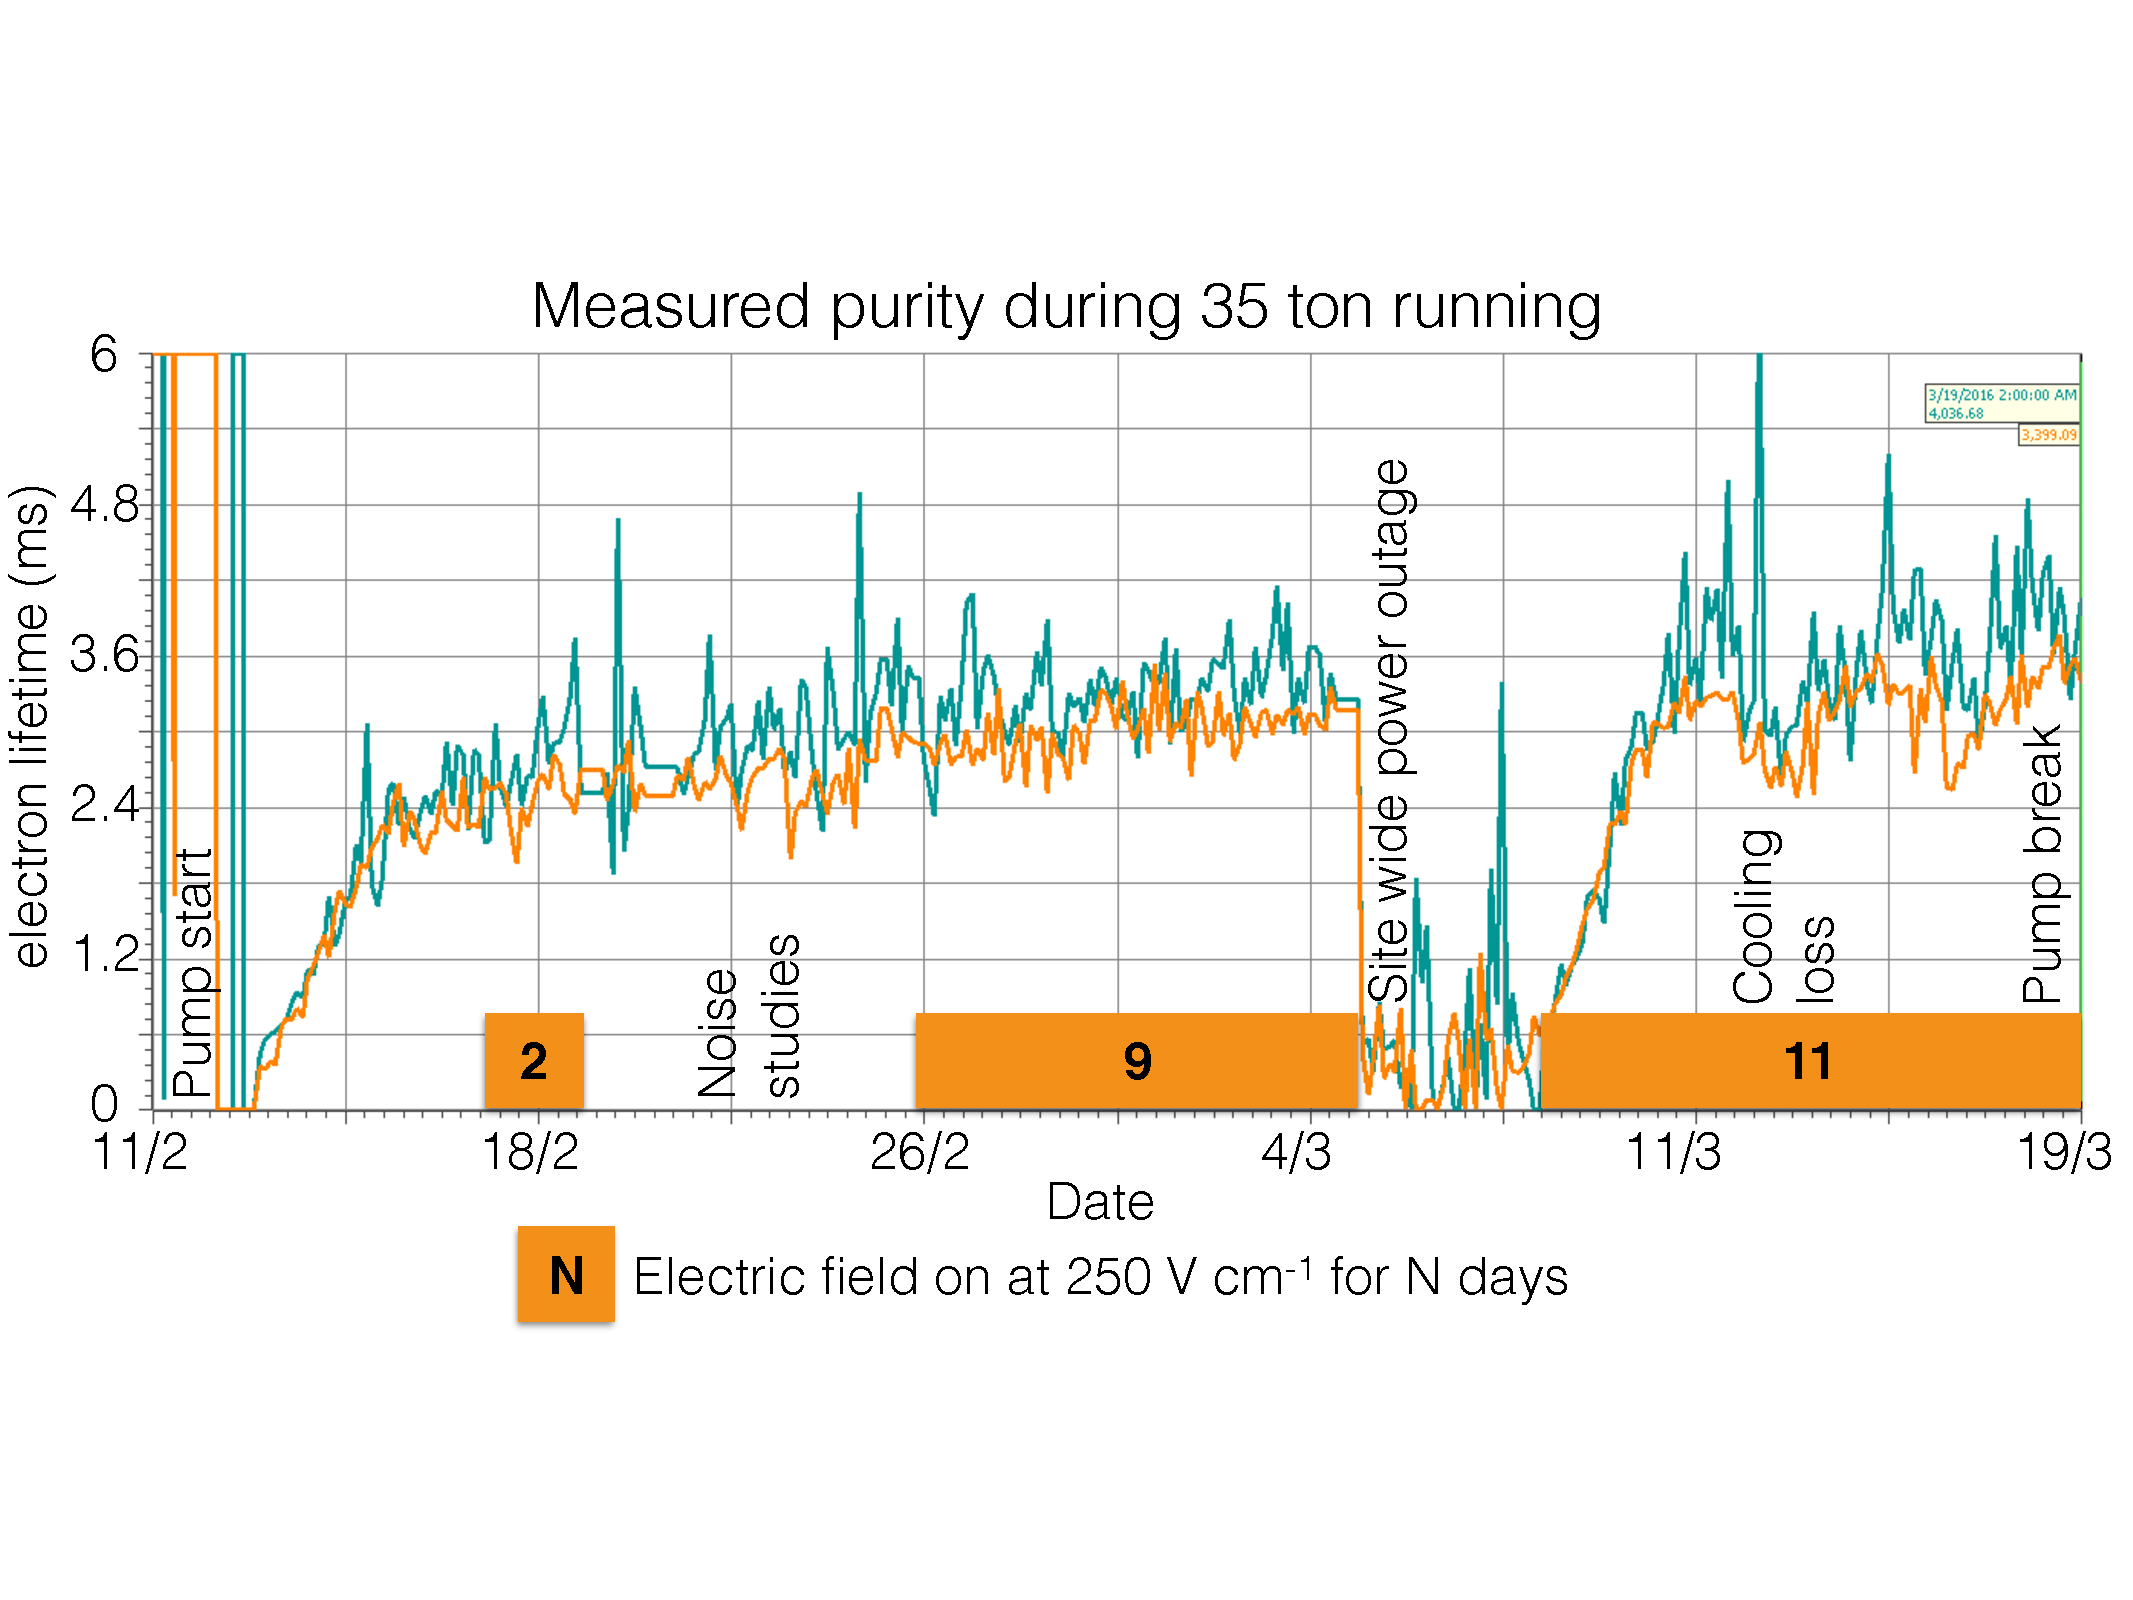
\includegraphics[width=1.0\textwidth]{DataCollected}
  \caption[The 35 ton data sample]{Timeline showing the data collected during the 35 ton Phase II run once the purification pumps were turned on.}
  \label{fig:DataCollected}  
\end{figure}


%********************************** %First Section  **************************************
\section{Organisation of the data structure} \label{Organisation of the data structure} %Section - X.1
As previously noted the 35 ton consisted of three detector sub-systems: RCEs collecting TPC data, SSPs collecting photon detector data, and CRCs collecting cosmic muon coincidences. The DAQ combined these three data streams into synchronous events in time saved as LArSoft objects called artdaq::Fragments. These data objects would later have to converted to the offline data products which the reconstruction tools developed on simulation used, this is discussed in \ref{Reformatting the data to the offline structure}. This section describes the structure of the data objects in the raw form.\\

During operations the DAQ was configured to maximise throughput and physics potential. This meant recording different lengths of times for each of the three sub-systems as the data volumes were significantly different. The maximum speed at which data could be written to disk was approximately 60 MB s$^{-1}$, this was roughly equal to the size of each triggered event when the entire detector was read-out in the configuration discussed below and so the 35 ton recorded events at roughly 1 Hz.\\

With an electric field of 250 V cm$^{-1}$ and a drift of 2.25 m, the drift time for electrons at the long drift CPA was roughly 2.6 ms or 5200 ticks (where 1 tick is 500 ns). It was decided that in order for a track causing a counter co-incidence to be separated from other tracks it was necessary to have one drift window both before and after the drift window around the co-incidence, meaning that data was recorded for 7.5 ms or 15,000 ticks around each co-incidence. The rate at which events were recorded could have been increased if zero-suppression had been used as data from the TPC was the dominant data being written out, however the elevated noise level meant that this was not feasible and so all ADC samples were recorded for all triggered events. The next most significant data volume was due to the SSPs which recorded data for XXXX $\mu$s around the trigger as this allows for the prompt light from the through-going particle to be collected. A larger time sample was not recorded to limit the data volume. The CRCs produced the least volume of data and so were able to be read out constantly, though the co-incidence triggers were only produced when a trigger was issued. The system used to collect the CRC data was also responsible for generating the triggers and so this meant that the production of triggers could be suppressed by only producing a trigger on the N$^{th}$ co-incidence. Without this feature the event rate would have been significantly higher, as the flux from muons triggering the vertical counters would have been over 60 Hz, before considering the horizontal co-incidences. \\

The time synchronous events produced by the DAQ did not however correspond to the physics events, this is because the DAQ was originally designed to produce a continuous data stream. This meant that the DAQ was configured to pad events with headers when there was a sub-system provided no physics information. Removing these padded header objects was a further remit of the online to offline converter discussed in \ref{Reformatting the data to the offline structure}. The length of the DAQ events was configurable and was chosen to be 10 ms (20,000 ticks) in order to best attempt to fully contain physics events and reduce the need for the online to offline converter to stitch DAQ events together. The padding of DAQ events with headers between physics events introduced some peculiarities in the data recorded such as DAQ events containing two parts of non-continuous data as shown in Figure~\ref{fig:DataStructure} where the second DAQ event has no information for time between the end of physics event 2 and the start of physics event 3.\\

\begin{figure}[h!]
  \centering
  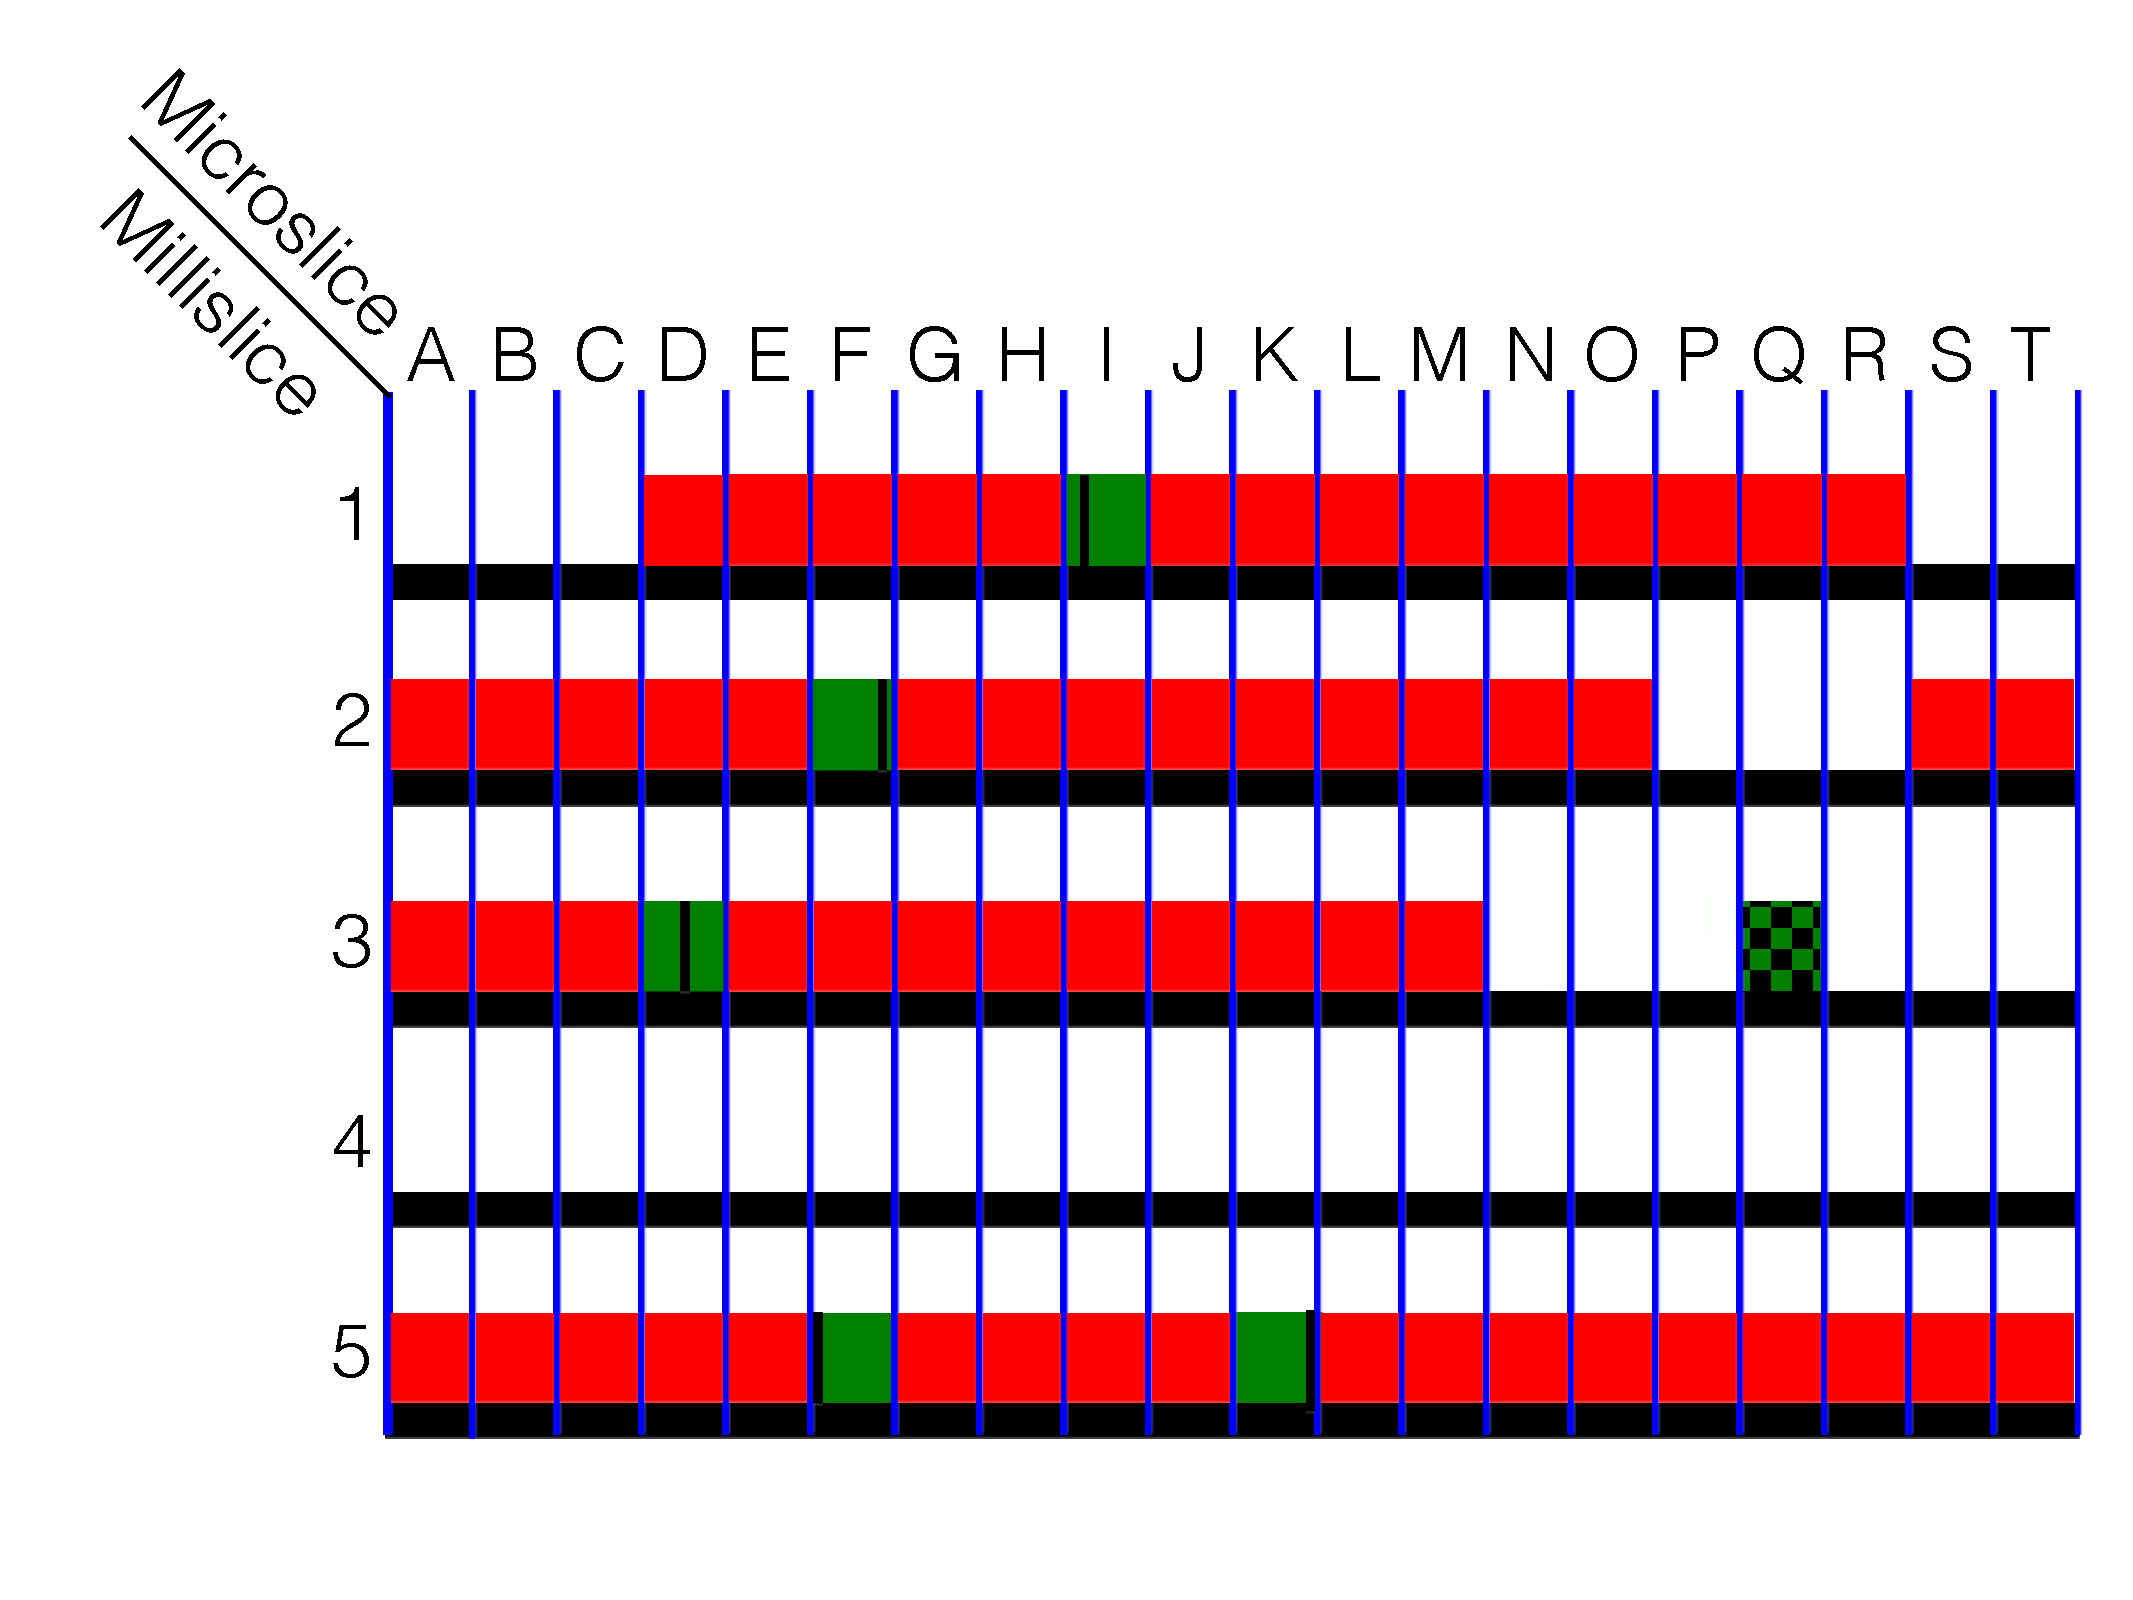
\includegraphics[width=0.75\textwidth]{DataStructure}
  \caption[The 35 ton data structure]{A diagram of possible microslice structures for the TPC data recorded by the 35 ton. Each row represents a single DAQ event. The vertical blue lines delineate each microslice (0.5 ms, 1,000 ticks). Solid red boxes represent micro slices with TPC data in them. Green boxes represent triggers which were used with the black lines showing the time at which the trigger occurred, and dashed green and black boxes represent triggers which were ignored.}
  \label{fig:DataStructure}
\end{figure}

As the run mode required accessing buffered data it had to be discretised inside the components before being sent to the event builders in the DAQ. In the discussion of how this worked focus will be given on the RCE data where some new terms need to be introduced. Data is collected for every tick on each RCE, where each RCE controls 128 channels. This is called a nanoslice. A microslice is then made by combining N nanoslices such that it contains 0.5 ms (1,000 ticks) of data across all channels. Microslices are then combined to make millislices, where a millislice is synonymous with the DAQ events discussed earlier meaning that 20 microslices are combined to make a millislice. A lack of recorded data means that microslices consist of headers in the place of nanoslices. \\

During normal data taking the last N microslices are buffered in the RCEs so that if a trigger is issued the previous millislices can be accessed before they are deleted. As the data is buffered in the form of microslices previous millislices may only be accessed in whole. This means that a whole number of millislices must be loaded before the trigger so when a trigger is issued part way through a millislice the previous X millislices are sent to the event builders. As a result during there are always a minimum number of ticks both before (5,000 ticks) and after the trigger (9,000 ticks) but the exact numbers can change by up to 1,000 ticks for a given event depending on where in a millislice the trigger comes. This is shown in Figure~\ref{fig:DataStructure} where the black lines representing triggers are seen to occur at different points within the microslices, for example physics event 1 will have more data after the trigger than physics event 2 as the trigger occurs earlier in the triggered microslice. \\

The information in this section has been summarised in FigureXXX and FigureXXX below.

%********************************** %Second Section  *************************************
\section{Reformatting the data to the offline structure} \label{Reformatting the data to the offline structure} %Section - X.2
Conversion of the raw data in the form of artdaq::Fragments to LArSoft objects such as raw::RawDigits (TPC), raw::ExternalTrigger (CRC) and recob::OpDetWaveforms (SSP) required a suite of unpacking services to be written; the specifics of which are not discussed here. These all required a common interface through which to access the data, check that the timing of each component was consistent and then produce a final LArSoft file for downstream use. This programme had the added role of producing complete physics events, meaning that it had to be able to combine multiple millislices and extract only the data containing the continuous physics events. \\

The format that the data reformatter followed was that following the unpacking of each of the sub-systems the TPC ticks would be looped through to see if a user defined set of conditions could be satisfied. These conditions were usually whether an East-West or North-South counter-coincidence occurred at that time, or if the current millislice contained TPC data whilst the previous one did not. The latter was the default configuration as this gave the option of preserving all of the data gathered, for reasons discussed at the end of \ref{Organisation of the data structure}. Other conditions were available though rarely used such as if a threshold of recob::OpDetWaveforms was exceeded or if there was a large change in average ADC value, corresponding to a large flash of light or an artificially induced signal on the wires respectively. Once a set of conditions is satisfied a user defined number of pre-condition ticks are gathered, clearly this is set to zero in the case of the previous millislice containing no TPC data as there is no previous data to load which would not have a gap in time, see Figure~\ref{fig:DataStructure}. In the case of using a counter co-incidence to make an event a value of 300 pre-condition ticks is normally used. Once the pre-conditions ticks are gathered a further N post-condition ticks are gathered, where N is defined by the user. Usually 15,000 ticks are gathered when the previous millislice is empty and 5,200 ticks are gathered when there is a co-incidence. Data from the other components is added to the event if its timestamp is within the timestamps of the first and last ticks in the event when no more TPC data is required from or can be gathered from the current millislice. All timestamps were then corrected such that the event began at T=0 as the reconstruction assumes this, the start time of the event was then stored in the event record so that it could be accessed downstream. \\

At all points in this process it is important to integrate flexibilty so that the user can choose the length of events, which sub-systems are in the events and what the conditions are for making events. It was also important for users to be able to run the service on already formatted events as the unpacking services were the major overhead in running the service, and it is also conceivable that users would want to reformat Monte Carlo events so as to centre them around their chosen conditions.

%********************************** % Third Section  *************************************
\section{Observations on data quality and noise mitigation} \label{All the noise} %Section - X.3
Reformatting the online data to the offline format was an important step in maintaining data quality as subsequently there was no access to the raw data due to how the DUNE software is established. Some of the important checks which were performed are outlined in Figure~\ref{fig:DataDrops}. If any of these issues were present in a given physics event then it is discarded as the integrity of the data cannot be gauranteed. It was decided that these events would be discarded as non-synchronous events would lead to hits in the detector being at incorrect times and padding empty events with pedestals could mean that tracks seem to dissapear as they travel through the detector. \\

DO I WANT A PLOT SHOWING HOW OFTEN THIS OCCURED??? \\

Another example of inconsistent events is when the sub-systems are not synchronised with eachother, this is normally caused by one of the sub-systems missing a clock increment from the master timing unit due to the data trigger being issued close to an increment from the master unit. This misallignment causes an incorrect time sample being read out and so the data from each sub-system within a millislice is not consistent meaning that it will fail the timestamp check and so won't be added to the event record. To avoid incomplete events the physics events are discarded when this is observed. \\

DO I WANT A PLOT SHOWING HOW OFTEN THIS OCCCURED?? \\

\begin{figure}[h!]
  \centering
  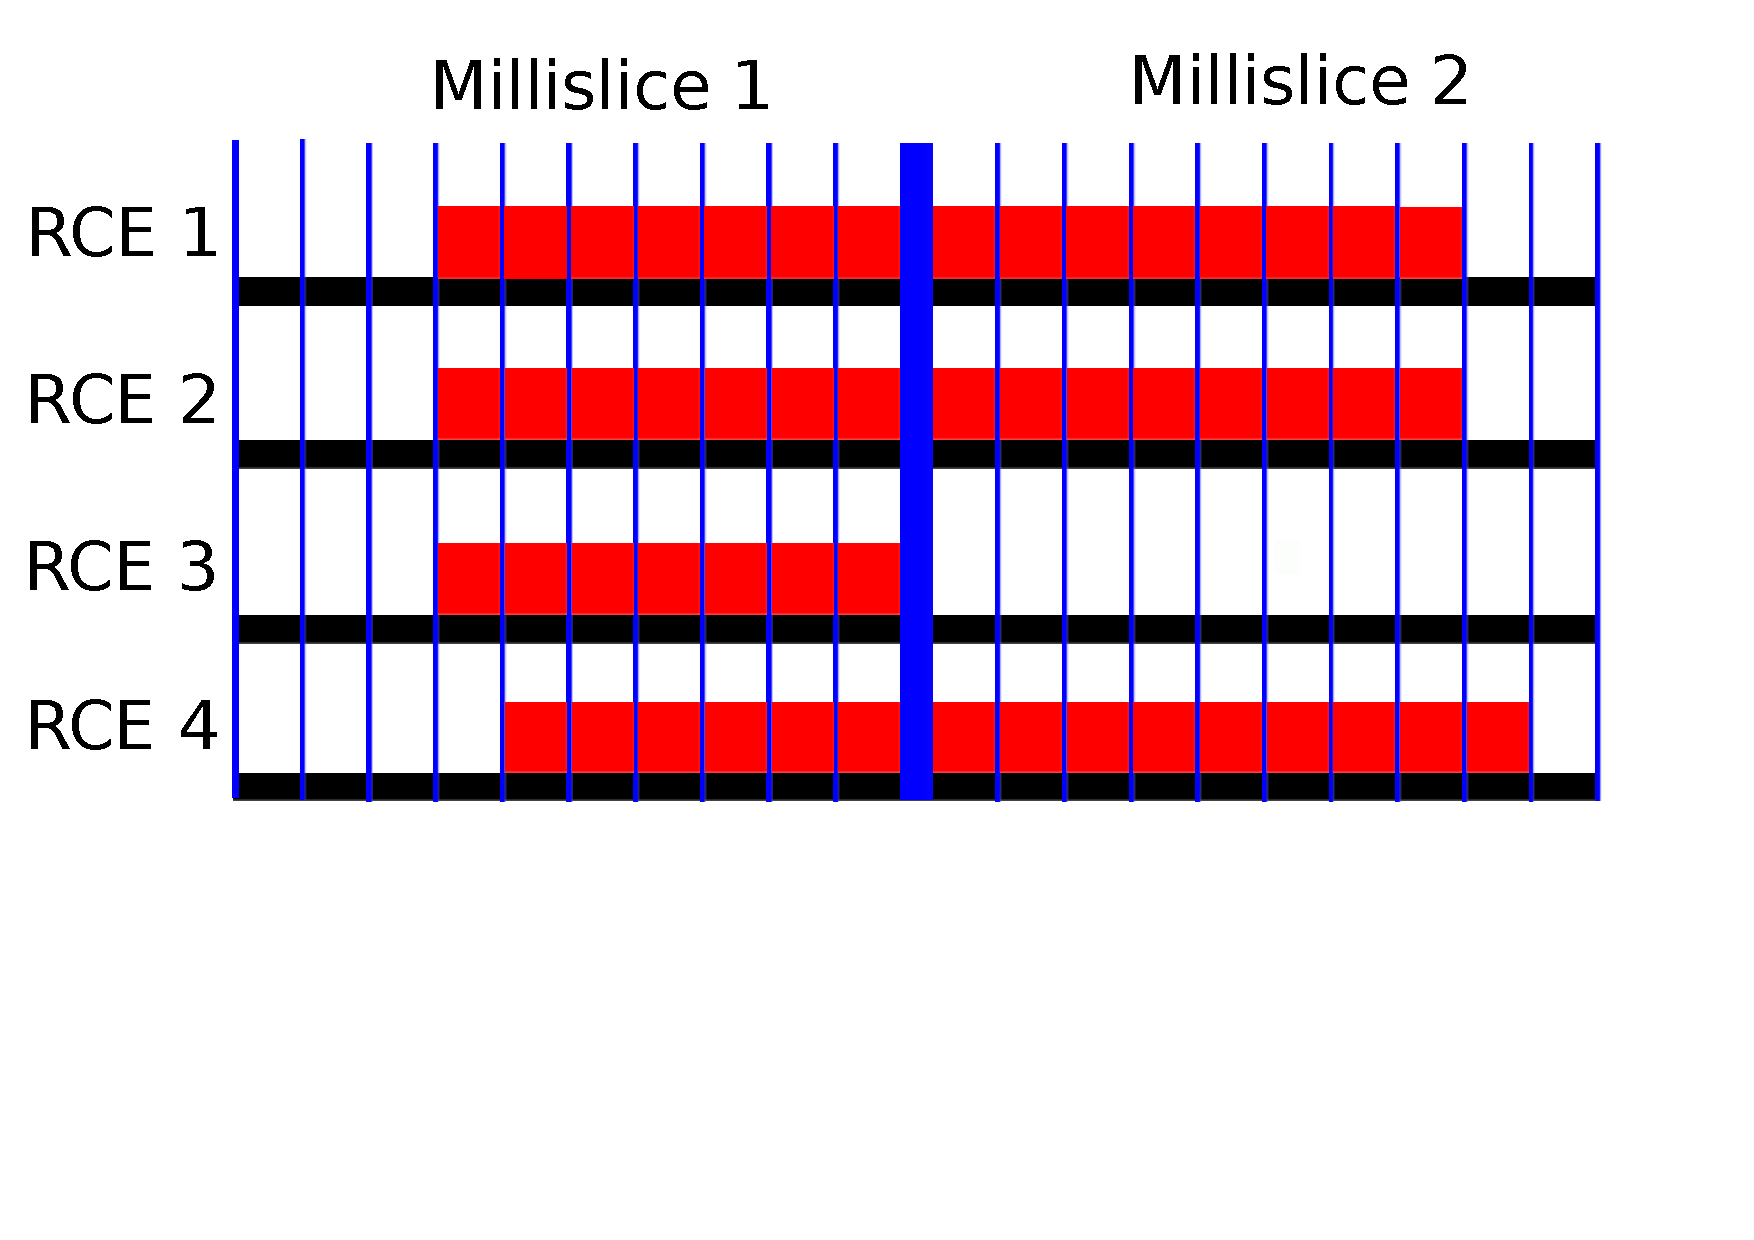
\includegraphics[width=0.85\textwidth]{DataDrops}
  \caption[Dropped TPC data in the 35 ton]{A diagram of how TPC microslices can be saved in millislices in the 35 ton. Two millislices are shown, each containing 10 microslices. One physics event straddling the millislice boundaries is shown and 4 RCEs representing each row are read out. The vertical blue lines delineate each microslice (0.5 ms, 1,000 ticks), with the thick blue line showing the millislice boundary. Solid red boxes represent micro slices with TPC data in them. It can be seen that RCEs 1 and 2 contain data for the same interval, whilst the data from RCE 3 in millislice 2 has been ``Dropped,'' whilst the data from RCE 4 is shifted by 1 microslice from RCEs 1 and 2 and is thus ``Inconsistent.'' As a result this physics would be discarded as data integretity cannot be gauranteed.}
  \label{fig:DataDrops}
\end{figure}

The electronic noise in the 35 ton was higher than anticipated, with the RMS of the RCE ADC being approximately 30 counts compared to an expected thermal noise of around 2.5 ADC counts. Many sources which are explained below contributed to this elevated noise. \\

Though not directly affecting the noise issues stuck ADC codes were a feature of the data which had to removed downstream. Stuck ADC codes were caused by the 6 least significant bits getting frozen to either 000000 or 111111, this was observed during the first stages of commisioning and an algorithm to remove them was developed and tested on Monte Carlo by Jonathan Insler of LSU. It was observed that in simulation the signal could be recovered with minimal losses, as shown in Figure~\ref{fig:StuckCodes} where the blue line (after removal) is seen to closely match the black line (before adding stuck codes). \\

A significant portion of the noise was correlated between groups of 32 channels, where the ADCs would coherently oscillate. To remove these coherent shifts ADC baselines were calculated for the 32 channel groups at each tick and then subtracted from the measured ADC values. This was also found to be an effective method of removing coherent noise in MicroBooNE \citep{uBooNENoise}. The effect of removing coherent noise is shown in Figure~\ref{fig:CoherentNoise}, where the signal peak becomes much easier to discern after noise removal. Subtracting increases in signal at a common time across adjacent wires reduces the signal strength of events which are parallel to the APAs however as the hits from these tracks will occur at roughly the same time. The only way to prevent this is to ``protect'' potential signal regions from the coherent noise removal, as is done in MicroBooNE \citep{uBooNENoise}. \\

When a Fast Fourier Transform (FFT) \citep{CoTuFFT} is performed on the coherent noise subtracted waveforms it can be seen that signals occur with specific frequencies. Some of these frequencies are caused by real energy depositions, whilst others are due to electronics noise. It is possible to remove the noise frequencies by applying Wiener filters \citep{WienerFilter}. For each of the three planes frequency spectrums are taken where a clear signal is both preserved and suppressed, the signal spectrum is then divided by the signal suppressed spectrum to produce a $signal/noise$ frequency space. The signal regions which want to be excluded can then be found by fitting a combination of sigmoid functions to the frequency spaces, a demonstation of how this applied is shown in FigureXXXXX. It is also possible to remove specific frequencies which are not removed by the filters, this was neccessary for a 54 KHz noise component introduced by the flourescent lights in the detector hall to be removed. After the run ended it was found that some of the high frequency noise components were introduced by a short on a warm power cable, the techniques used to find this cable will be used then commisioning future detectors \citep{35tonNoiseMeeting}. \\

WANT PLOTS OF APPLYING THE FREQUENCY FILTERS!!!! \\

\begin{figure}[h!]
  \centering
  \begin{minipage}{0.45\textwidth}
    \centering
    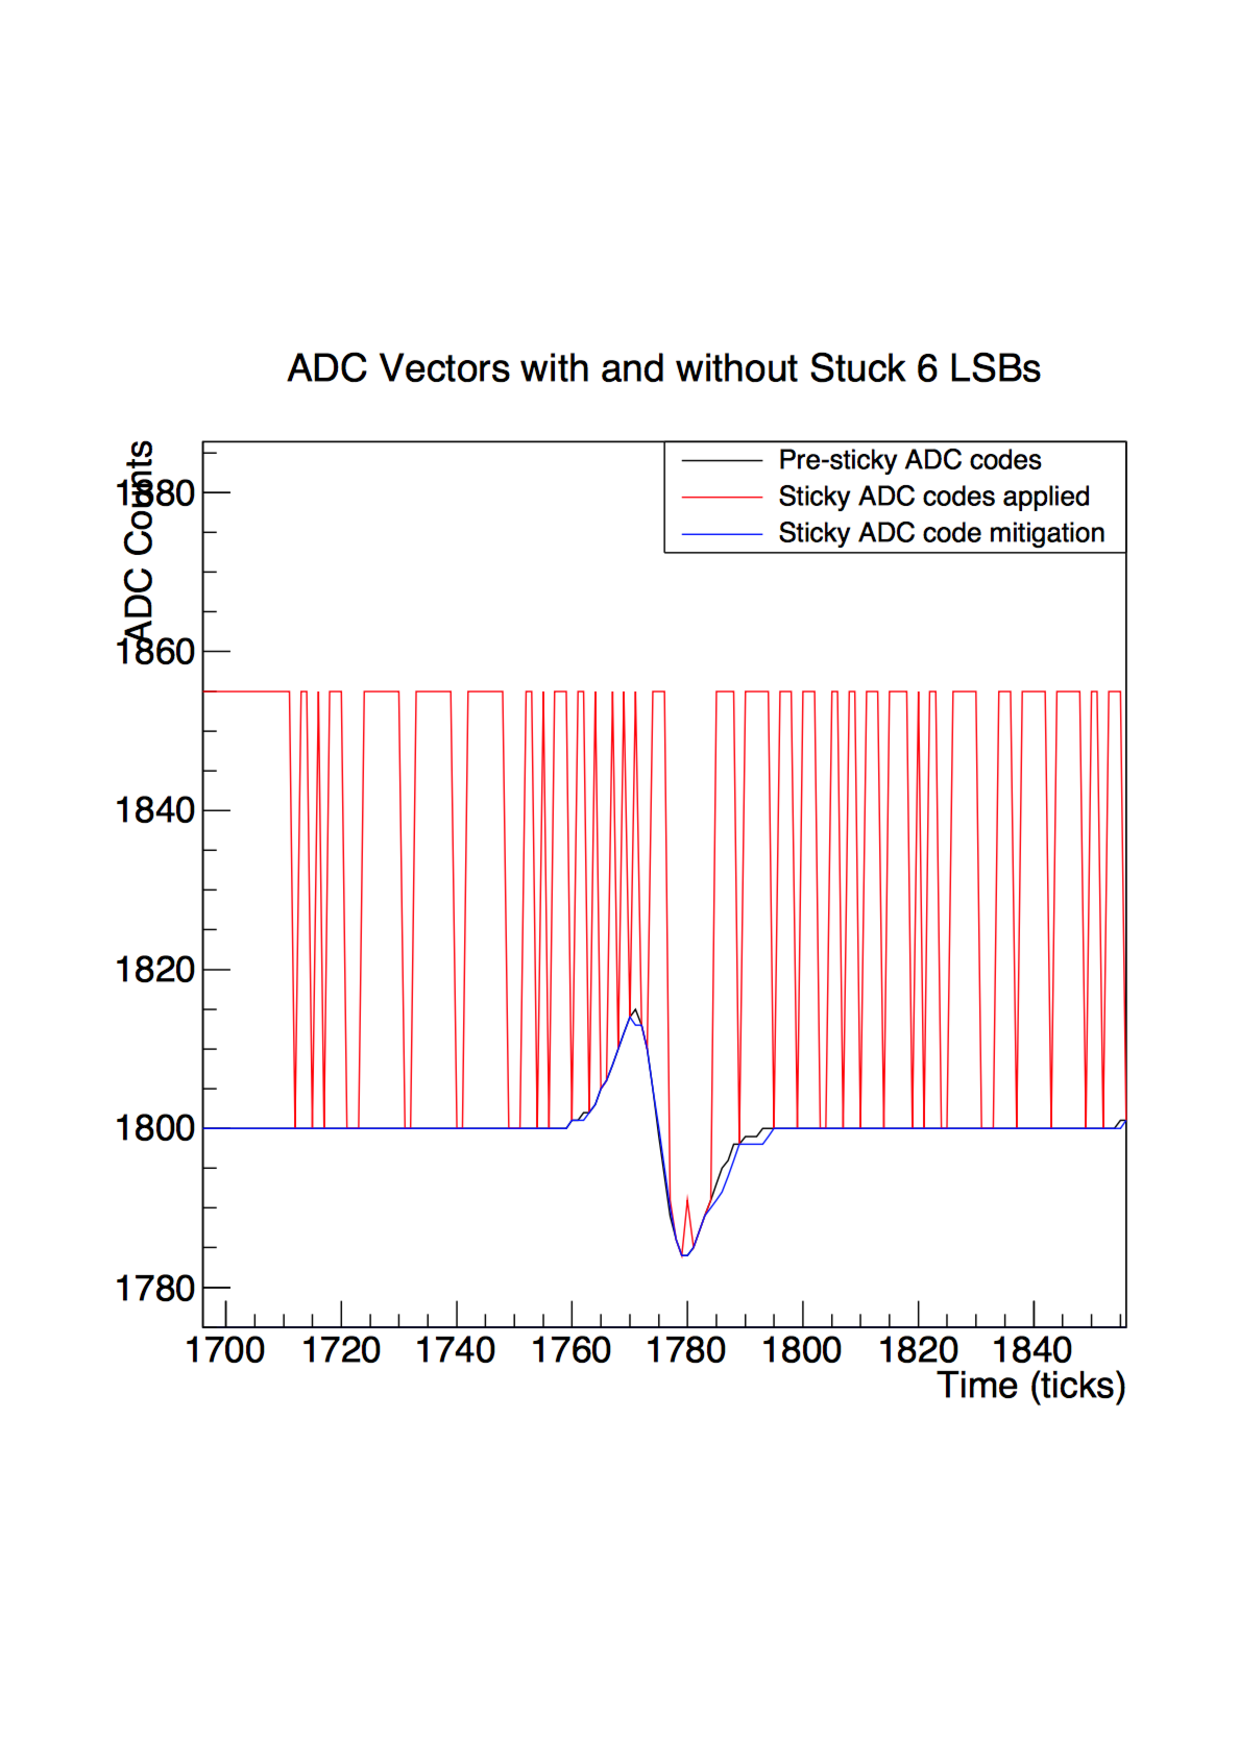
\includegraphics[width=\textwidth]{StuckCodes}
  \end{minipage}
  \begin{minipage}{0.45\textwidth}
    \centering
    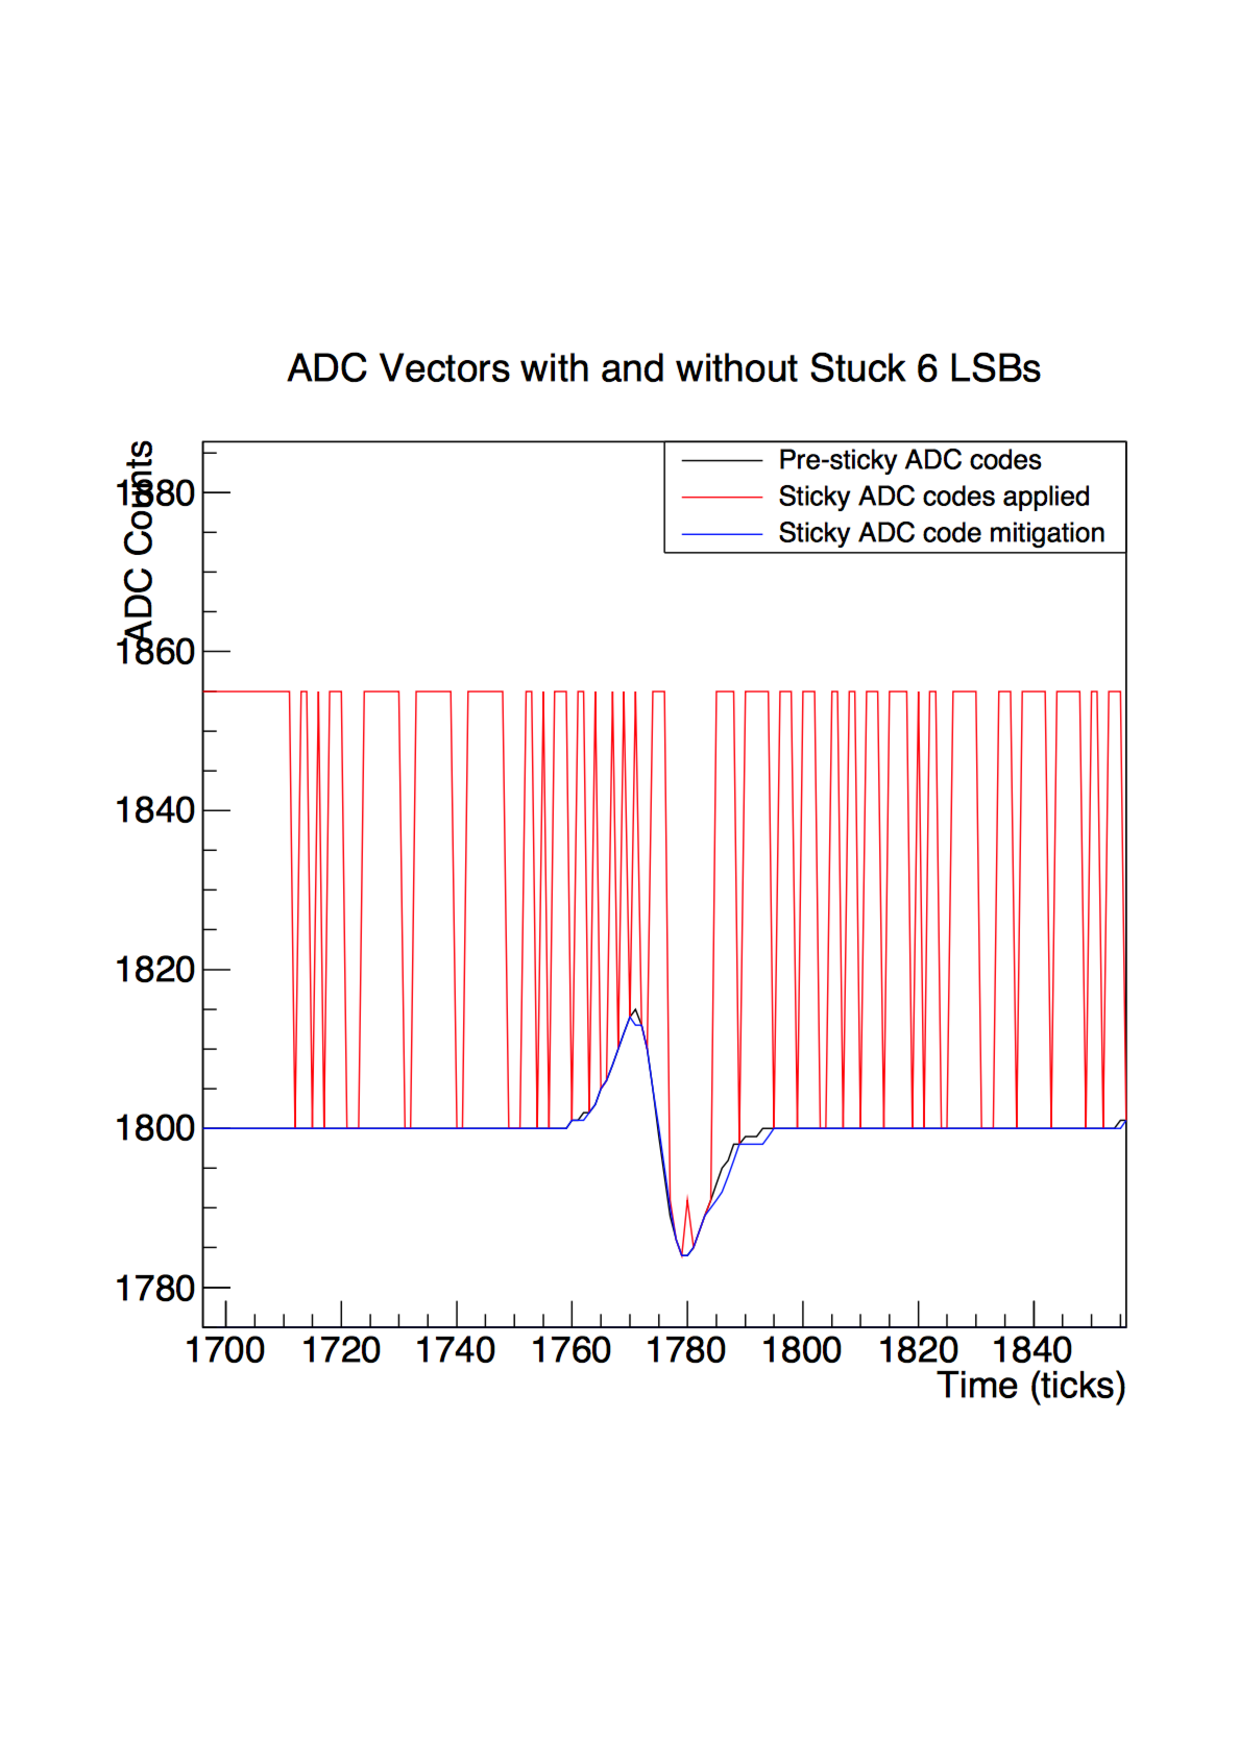
\includegraphics[width=\textwidth]{StuckCodes}
  \end{minipage}
  \caption[Recovering stuck ADC codes in the 35 ton]{Two Monte Carlo spectrums showing the effect of the introduction and removal of stuck bits on a simulated signal \citep{InslerStuckCode}.}
  \label{fig:StuckCodes}
\end{figure}

\begin{figure}[h!]
  \centering
  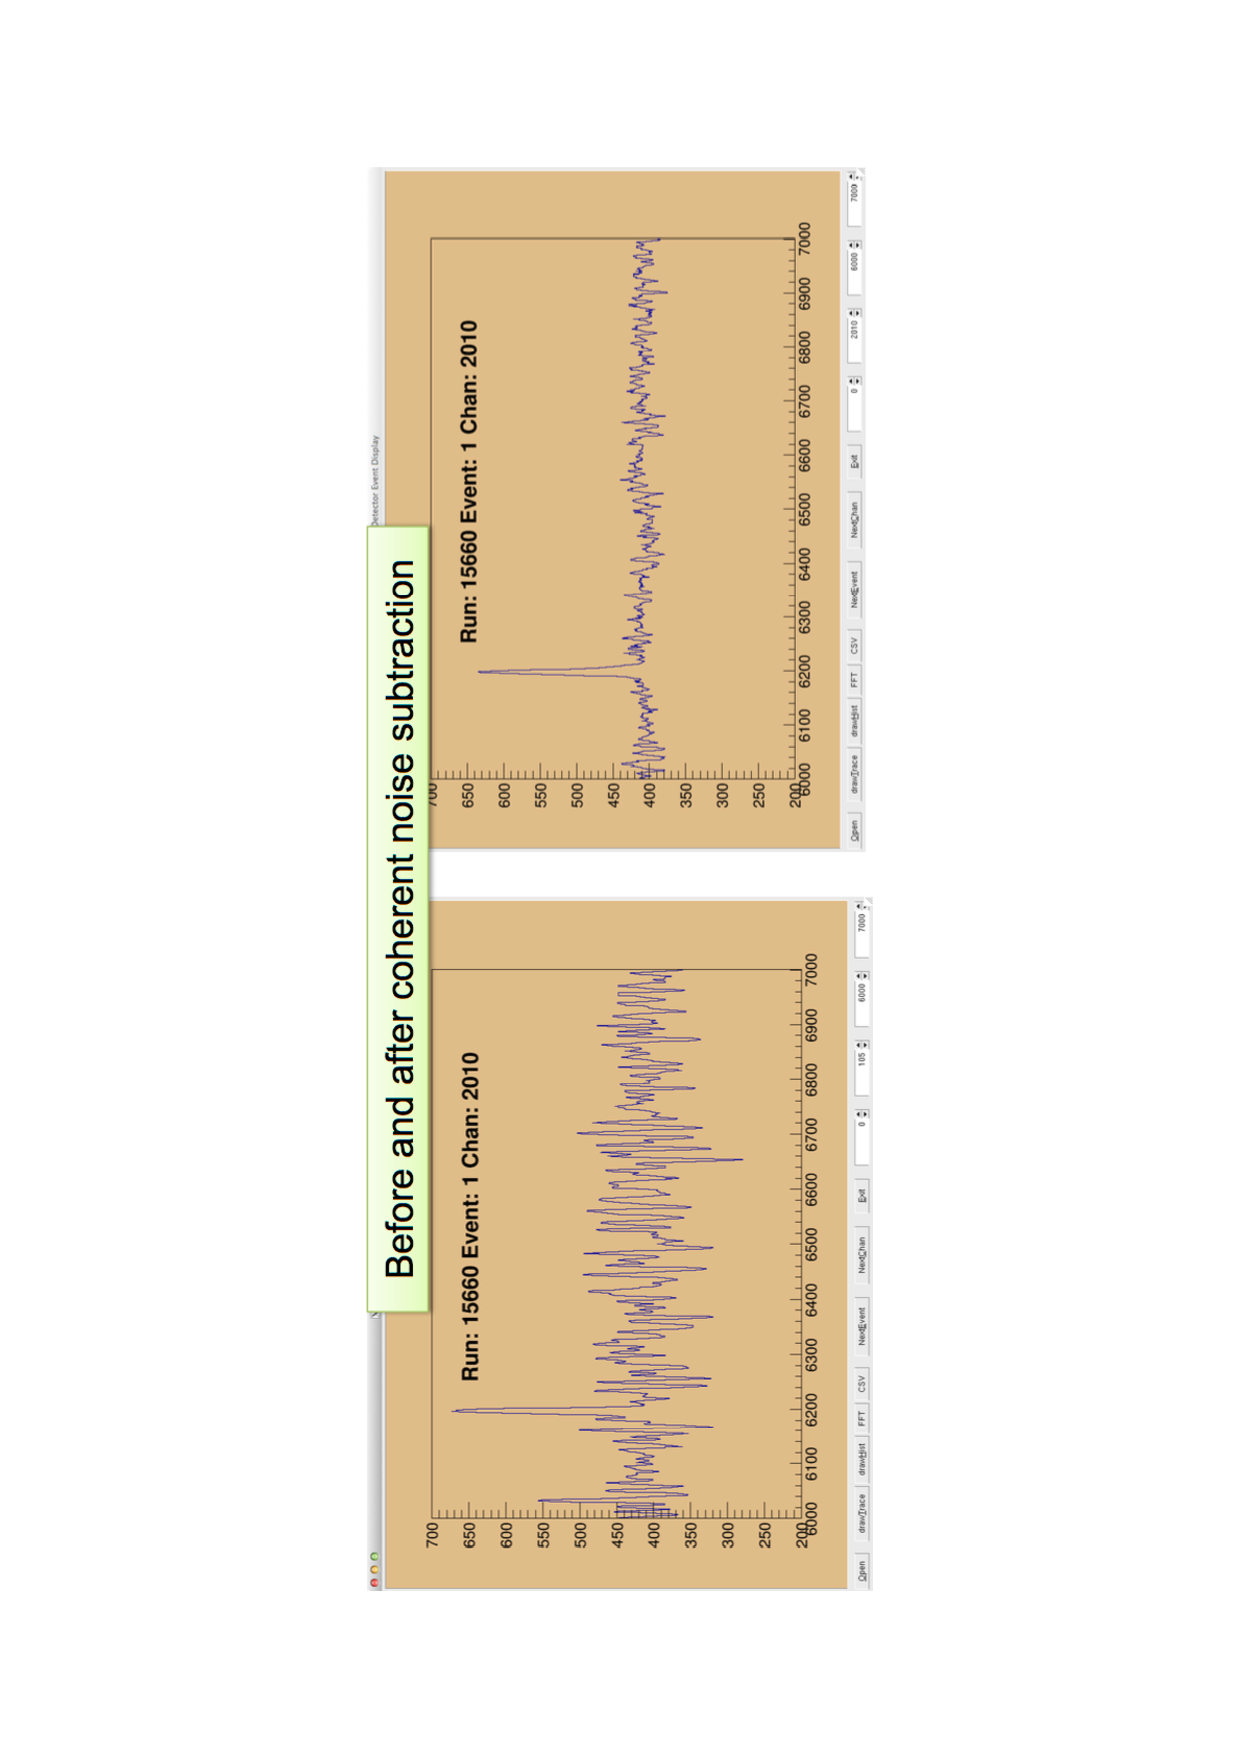
\includegraphics[width=\textwidth]{CoherentNoise}
  \caption[Removing coherent noise in the 35 ton]{Plot showing the effect of the removing coherent noise on a real signal.}
  \label{fig:CoherentNoise}
\end{figure}

An example of the effect of the noise mitigation steps is shown in FigureXXXXX, where the left side shows the raw data and the right side shows the data after the stuck code unsticker, coherent noise removal and Wiener filter algorithms have been applied after the removal of noisy wires. \\

Transitions to a higher noise level state were also observed after cooldown. The transitions would seemingly occur at random, but were occasionally observed to happen shortly after a saturation event across the whole detector \citep{35tonNoiseMeeting}. After the transition the only way to recover the normal noise state was to power down the TPC components on APA 3, this was the only APA which did not have a ground mesh between the two sets of wire planes which may offer some clue to the cause of the effect though it could not be induced during warm testing and has not been observed in other experiments such as MicroBooNE. The elevated noise state was associated with a strong signals at high frequencies, between 400 and 650 KHz. The values of these frequencies changed during the run as shown in FigureXXXX, though once a transition at a given frequency was induced it did not change until the TPC components were powered down. Data taken during these events was unrecoverable as the noise was too large, as such upon observing a transition the TPC components were quickly power cycled. 

%********************************** % Fourth Section  *************************************
\section{Performance of reconstruction algorithms}  %Section - X.4
Following the noise removal outlined above hit and track finding was still more difficult than in simulations due to the still elevated noise level. In order for a sensible number of hits to be reconstructed the hit finding threshold had to be substantially increased in data as compared to Monte Carlo, this meant that many of the low energy hits would not be reconstructed. \\

A potential solution to not reconstructing the low energy hits is to use the counter positions to select only hits which could have caused co-incidences. When determing whether a reconstructed hit could have caused the counter-coincidence a two-dimensional window around the counter edges is constructed and timing information is used to extend this to three dimensions.  The X position of the hit can be calculated using the hit time and electron drift time using \ref{eq:HitTime}. \\
\begin{equation} \label{eq:HitTime}
  X_{Hit} = T_{Hit} \times V_{Drift}
\end{equation}

Determining whether collection plane hits are within the counter window is trivial as they have a constant Z position and either cover the full detector height (tall APAs) or roughly half of the detector height (short APAs). The wrapping of the induction planes means that each wire segment has to be considered individually and that multiple wire segments could lie within the counter shadow. Choosing between these potential wire segments is done by iterating through the following steps, if at any point only one segment satisfies the condition then this segment is chosen:
\begin{itemize}
\item Does the wire segment intersect any collection plane wires which record hits?
  \begin{itemize}
  \item This is because when there is a signal on the collection plane there should also be signals on the induction wires.
  \end{itemize}
\item Are there adjacent wires which have hits at a similar time?
  \begin{itemize}
  \item This is because one would expect a track to deposit energy on multiple adjacent wire segments. 
  \end{itemize}
\item Which hit lies closest to the line defined by unqiue collection plane hits in the XZ plane?
  \begin{itemize}
  \item This is follows identical logic to the first criteria, but selects the hit which best matches the line and attempts to remove the effect of noisy collection plane wires by only using wires which have one hit within the counter shadow. This would also hopefully improve the quality of the fit as there will not be numerous outlying hits.
  \item This can be changed to consider the line defined by previously selected hits in the given TPC and plane where the hit choices are.
  \end{itemize}
\end{itemize}
DO I WANT SOME SORT OF FIGURE SHOWING THIS? LOTS OF HITS -> ONLY TRACK HITS? COL HITS USED IN ITEM 3, OVERLAYED WITH ALL INDUCTION PLANE HITS CONSIDERED, WITH THE ONES KEPT IN A DIFFERENT COLOUR? \\

Following a re-optimisation of the clustering algorithms it was observed that the standard reconstruction could achieve track reconstruction to a similar efficiency as the counter shadowing and so the standard reconstruction has been used in the discussions to follow \citep{TingjunClustering}. There has since been an effort to improve the counter shadowing hit disambiguation to remove the outlying collection plane hits using a <<ASK MATT FOR ONE LINE SENTENCE SUMMARISING HIS STUFF>>.\\

%****** Now to talk about the reconstruction efficiencies... ******%



%********************************** % Fifth Section  *************************************
\section{???Measuring interaction times using electron diffusion???}  %Section - X.5

